\documentclass{beamer}
%% Possible paper sizes: a0, a0b, a1, a2, a3, a4.
%% Possible orientations: portrait, landscape
%% Font sizes can be changed using the scale option.
\usepackage[size=a3,orientation=portrait,scale=1.8]{beamerposter}
\usetheme{LLT-poster}
\usecolortheme{ComingClean}
% \usecolortheme{Entrepreneur}
% \usecolortheme{ConspiciousCreep}  %% VERY garish.

\usepackage[utf8]{inputenc}
\usepackage[T1]{fontenc}
\usepackage{libertine}
\usepackage[scaled=0.92]{inconsolata}
\usepackage[libertine]{newtxmath}
\usepackage[numbers]{natbib}
\renewcommand{\bibfont}{\small}

\newcommand{\texthash}{\#}


%% Load the markdown package
\usepackage[citations,footnotes,definitionLists,hashEnumerators,smartEllipses,tightLists=false,pipeTables,tableCaptions,hybrid]{markdown}
%%begin novalidate
\markdownSetup{rendererPrototypes={
 link = {\href{#2}{#1}},
 headingFour = {\begin{block}{#1}},
 horizontalRule = {\end{block}}
}}
%%end novalidate

\author[Chevalier.V]{mecacorbu.odoo.com/}
\title{STS CPRP $1^{ere}$ année}
\institute{Lycée Le Corbusier}
% Optional foot image
\footimage{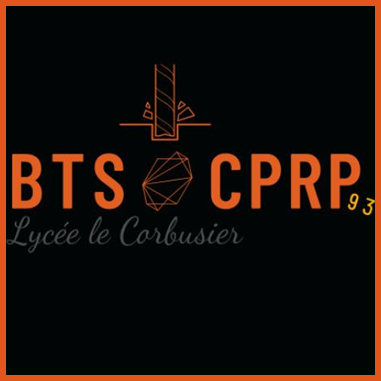
\includegraphics[width=4cm]{logo1.png}}

\begin{document}

\begin{frame}[fragile]\centering

\textbf{\textit{Document de rentrée scolaire}}

\begin{columns}
\begin{column}{0.57\textwidth}

\begin{markdown}

#### Fournitures

- Trousse de crayons de couleurs
- Agenda (numérique ou autre, google etc.)
- Crayon à papier/Critérium/Porte mine
- Classeur/trieur avec pochettes plastiques/intercalaires
- Clef USB $> 10$ Giga 
- Calculatrice classique


----
\end{markdown}
\end{column}


\begin{column}{.4\textwidth}
\begin{markdown}




#### Fourniture accès libre

- Règles, compas, équerres, pieds à coulisse
- Blouse, chaussures de sécurités (avec casiers)
- Dossier personnel sur le réseau local du lycée



----
\end{markdown}
\end{column}

\end{columns}

\bigskip
{\usebeamercolor[bg]{headline}\hrulefill}
\bigskip

\begin{columns}[T]

%%%% First Column
\begin{column}{.46\textwidth}

\begin{markdown}

#### Toujours travailler sur son réseau

- Au lycée, on distingue deux grandes structures, le réseau commun et le \textbf{réseau personnel}. Le réseau commun contient trois sous dossiers : "\textit{ Document en consultation}" (vous pouvez prendre des dossiers/fichiers), "\textit{Espace d’échange}" (vous pouvez prendre ET déposer des dossiers/fichiers) et "\textit{Restituions des devoirs}" (vous pouvez seulement déposer des dossiers/fichiers).
- Vous devez toujours essayer de travail dans votre réseau personnel et non sur le réseau commun pour
éviter les problèmes de connexions ou de perte de réseau

----

#### Colour Themes

- I've include

---- 

#### Réseau du lycée

\setkeys{Gin}{width=.3\linewidth}

\begin{figure}
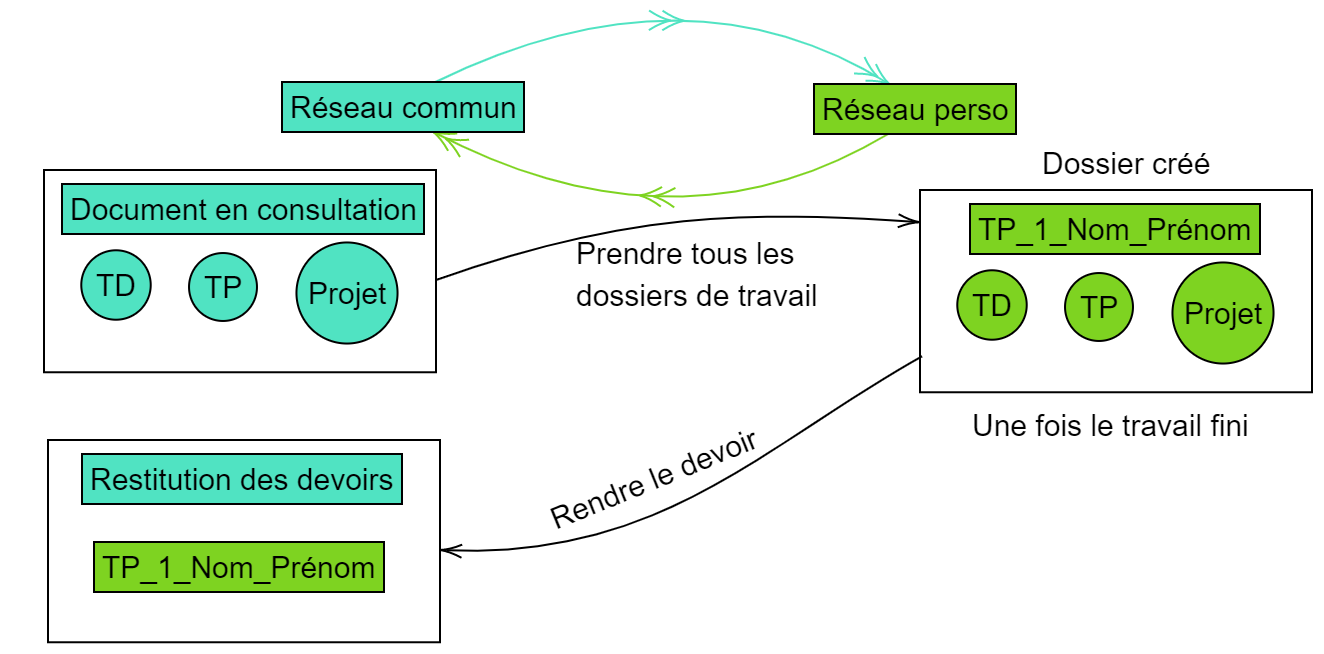
\includegraphics[width=1\textwidth]{A1.png} 
\end{figure}

----

\end{markdown}

\end{column}

%%%% Second Column
\begin{column}{.46\textwidth}

\begin{markdown}

#### Première connexion

- Un identifiant et un mot de passe vous seront donnés. Lors de votre première connexion, vous devrez \textbf{redéfinir un nouveau mot de passe}. Pensez à bien noté, ou \textbf{prendre en photo} l'identifiant et le \textit{nouveau mot de passe}, car il sera difficile de les récupérer rapidement.
- Five, six, pick up sticks
- Seven, eight, lay them straight
- Nine, ten, a big fat hen

----

#### Nommer ses fichiers

- D’une manière générale, vos fichiers doivent être compréhensible et identifiable. Nous devons savoir quel est le nom du devoir, et le ou les prénoms/noms. Si vous faite un devoir de dessin industriel, vous pouvez enregistrer vos devoirs de cette façon :

- \textbf{Dessin-definition-1-Nom-Prenom.catDrawing}

----


#### Enregistrement CATIA V5

Une attention particulière doit être prêter aux travail sur le logiciel. Vous devrez toujours nommer vos fichiers \textbf{SANS ACCENTS}, \textbf{SANS ESPACES}. Noté avec bon sens pour faciliter la compréhension. Vous aurez de \textit{nombreux} fichiers CATIA, il est important d'être directement bien organisé.e.

----

\end{markdown}
\end{column}
\end{columns}


\begin{markdown}

#### This is a sample of a wiiiide column

- One, two, pick up my shoe
- Three, four, shut the door
- Five, six, pick up sticks

----

\end{markdown}

\end{frame}


\end{document}